% ============================================================================
% !Document: DCR1 [zxweather Desktop Client]
% ----------------------------------------------------------------------------
% !Revision: 001
% !IssueDate: January 2013
% !Status: Unreleased
%
% !-Classification
% !ProjectCode: DAZW [Database Applications, zxweather]
% !Type: DCR [Desktop Client Reporting]
%
% !Copyright: (C) David Goodwin, 2018
% !License: FDL [GNU Free Documentation License]
% !Auhtor: David Goodwin
% ============================================================================

% Document information. This should match the above
\newcommand{\doctitle}{zxweather Desktop Client}
\newcommand{\docsubtitle}{Report Authoring}
\newcommand{\projectnum}{DAZW}
\newcommand{\docnum}{DCR1}
\newcommand{\docrev}{001}
\newcommand{\docdate}{August 2019}
\newcommand{\docauthor}{David Goodwin}
\newcommand{\docabstract}{This manual documents the zxweather desktop clients reporting system, cache schema and built-in reports.}
\newcommand{\docupdateinfo}{This is a new manual}
\newcommand{\docosver}{Linux; Microsoft Windows 7+}
\newcommand{\docswver}{zxweather 1.0}
\newcommand{\doccopyright}{\textcircled{c} Copyright David Goodwin, 2018, 2019.}
\newcommand{\doclicense}{Use, reproduction and modification of this document is permitted subject to the terms of the GNU Free Documentation License, Version 1.3 or any later vesion published by the Free Software Foundation. See \url{http://www.gnu.org/copyleft/fdl.html} for full license text.}

%%%%%%%%%%%%%%%%%%%%%%%%%%%%%%%%%%%%%%%%%%%%%%%%%%%%%%%%%%%%%%%%%%%%%%%%%%%%%
%                                 CONFIGURATION                             %
%%%%%%%%%%%%%%%%%%%%%%%%%%%%%%%%%%%%%%%%%%%%%%%%%%%%%%%%%%%%%%%%%%%%%%%%%%%%%

% Book type document, A4 paper, 10pt std font size:
%\documentclass[a4paper,10pt,draft]{book} 
\documentclass[a4paper,10pt]{book} 

\usepackage[scaled=0.90]{helvet} % Use helvetica as the standard font
\usepackage{courier}			 % Use courier as the fixed-width font
\usepackage{hyperref}			 % Links in PDF output
\usepackage{a4wide}				 % Narrower margins for A4 documents
\usepackage{ifthen}				 % A few if statements
\usepackage{multirow}			 % Column spanning in tables
\usepackage{graphicx}			 % For pictures
\usepackage{tabularx}			 % For customising table column types
\usepackage{listings}
\usepackage{gensymb}

 \usepackage{bera}% optional: just to have a nice mono-spaced font
 \usepackage{xcolor}
\usepackage{color}


% Configure JSON support in the listings package
% \colorlet{punct}{red!60!black}
% \definecolor{background}{HTML}{EEEEEE}
% \definecolor{delim}{RGB}{20,105,176}
% \colorlet{numb}{magenta!60!black}
%
% \lstdefinelanguage{json}{
%     basicstyle=\normalfont\ttfamily,
%     numbers=left,
%     numberstyle=\scriptsize,
%     stepnumber=1,
%     numbersep=8pt,
%     showstringspaces=false,
%     breaklines=true,
%     frame=lines,
%     backgroundcolor=\color{background},
%     literate=
%      *{0}{{{\color{numb}0}}}{1}
%       {1}{{{\color{numb}1}}}{1}
%       {2}{{{\color{numb}2}}}{1}
%       {3}{{{\color{numb}3}}}{1}
%       {4}{{{\color{numb}4}}}{1}
%       {5}{{{\color{numb}5}}}{1}
%       {6}{{{\color{numb}6}}}{1}
%       {7}{{{\color{numb}7}}}{1}
%       {8}{{{\color{numb}8}}}{1}
%       {9}{{{\color{numb}9}}}{1}
%       {:}{{{\color{punct}{:}}}}{1}
%       {,}{{{\color{punct}{,}}}}{1}
%       {\{}{{{\color{delim}{\{}}}}{1}
%       {\}}{{{\color{delim}{\}}}}}{1}
%       {[}{{{\color{delim}{[}}}}{1}
%       {]}{{{\color{delim}{]}}}}{1},
% }

\colorlet{punct}{red!60!black}
 \definecolor{background}{HTML}{EEEEEE}
 \definecolor{delim}{RGB}{20,105,176}
 \colorlet{numb}{magenta!60!black}

 \lstdefinelanguage{json}{
     basicstyle=\normalfont\ttfamily,
     numbers=left,
     numberstyle=\scriptsize,
     stepnumber=1,
     numbersep=8pt,
     showstringspaces=false,
     breaklines=true,
     frame=lines,
     backgroundcolor=\color{background},
     literate=
      *{0}{{{\color{numb}0}}}{1}
       {1}{{{\color{numb}1}}}{1}
       {2}{{{\color{numb}2}}}{1}
       {3}{{{\color{numb}3}}}{1}
       {4}{{{\color{numb}4}}}{1}
       {5}{{{\color{numb}5}}}{1}
       {6}{{{\color{numb}6}}}{1}
       {7}{{{\color{numb}7}}}{1}
       {8}{{{\color{numb}8}}}{1}
       {9}{{{\color{numb}9}}}{1}
       {:}{{{\color{punct}{:}}}}{1}
       {,}{{{\color{punct}{,}}}}{1}
       {\{}{{{\color{delim}{\{}}}}{1}
       {\}}{{{\color{delim}{\}}}}}{1}
       {[}{{{\color{delim}{[}}}}{1}
       {]}{{{\color{delim}{]}}}}{1},
 }


 \definecolor{lightgray}{rgb}{.9,.9,.9}
 \definecolor{darkgray}{rgb}{.4,.4,.4}
 \definecolor{purple}{rgb}{0.65, 0.12, 0.82}

 \lstdefinelanguage{JavaScript}{
   keywords={typeof, new, true, false, catch, function, return, null, catch, switch, var, if, in, while, do, else, case, break},
   keywordstyle=\color{blue}\bfseries,
   ndkeywords={class, export, boolean, throw, implements, import, this},
   ndkeywordstyle=\color{darkgray}\bfseries,
   identifierstyle=\color{black},
   sensitive=false,
   comment=[l]{//},
   morecomment=[s]{/*}{*/},
   commentstyle=\color{purple}\ttfamily,
   stringstyle=\color{red}\ttfamily,
   morestring=[b]',
   morestring=[b]"
 }

 \lstset{
    language=JavaScript,
    backgroundcolor=\color{lightgray},
    extendedchars=true,
    basicstyle=\footnotesize\ttfamily,
    showstringspaces=false,
    showspaces=false,
    numbers=left,
    numberstyle=\footnotesize,
    numbersep=9pt,
    tabsize=2,
    breaklines=true,
    showtabs=false,
    captionpos=b
 }


% use zxtechdoc styles if they're there
\IfFileExists{zxtitle.sty}{\usepackage{zxtitle}}{}
\IfFileExists{zxtechdoc.sty}{\usepackage{zxtechdoc}}{}

\hypersetup{
    unicode=false,          % non-Latin characters in Acrobat’s bookmarks
    pdftoolbar=true,        % show Acrobat’s toolbar?
    pdfmenubar=true,        % show Acrobat’s menu?
    pdffitwindow=false,     % window fit to page when opened
    pdfstartview={FitH},    % fits the width of the page to the window
    pdftitle={\doctitle{} - \docsubtitle},    % title
    pdfauthor={\docauthor},     % author
    pdfsubject={\doctitle},   % subject of the document
    pdfkeywords={\doctitle} {\docsubtitle}, % list of keywords
    pdfnewwindow=true,      % links in new window
    colorlinks=true,       % false: boxed links; true: colored links
    linkcolor=black,          % color of internal links
    citecolor=green,        % color of links to bibliography
    filecolor=magenta,      % color of file links
    urlcolor=black           % color of external links
}

% Build the partnumber. Format is PROJ-DOCU.REV. If revision is 001 then it 
% is not displayed. If project is undefined it is not displayed.
\newcommand{\partnumber}{\ifthenelse{\isundefined{\projectnum}}{}{\projectnum-\docnum	\ifthenelse{\equal{\docrev}{001}}{}{.\docrev}}}

% ragged-right paragraphs for tabular environments. Use 'P' instead of 'p'.
\newcolumntype{P}[1]{>{\raggedright\arraybackslash}p{#1}}

\newcommand*\cleartoleftpage{%
  \clearpage
  \ifodd\value{page}\hbox{}\newpage\fi
}

\begin{document}

% Roman Numerals for the front matter
\pagenumbering{roman}

% Setup the titlepage. We will use the zxtitle format if its there,
% otherwise the much simpler standard LaTeX one.
\ifthenelse{\isundefined{\ordernumber}}{

% Standard LaTeX titlepage
\title{\doctitle{} - \docsubtitle}
\author{\docauthor}
}{

% zxtitle titlepage
\title{\doctitle}
\subtitle{\docsubtitle}
\titleabstract{\docabstract}
\ordernumber{\partnumber}
\updateinfo{\docupdateinfo}
\osinfo{\docosver}
\swversion{\docswver}
\titlecopyright{\doccopyright}
\licensestatement{\doclicense}
}
\date{\docdate}

\maketitle

\clearpage

\tableofcontents
\clearpage

%%%%%%%%%%%%%%%%%%%%%%%%%%%%%%%%%%%%%%%%%%%%%%%%%%%%%%%%%%%%%%%%%%%%%%%%%%%%%
%                                 DOCUMENT                                  %
%%%%%%%%%%%%%%%%%%%%%%%%%%%%%%%%%%%%%%%%%%%%%%%%%%%%%%%%%%%%%%%%%%%%%%%%%%%%%

% Setup listings package



\lstset{
  frame=single,
  numbers=left,
  basicstyle=\small,
  commentstyle=\emph
}



\chapter{Introduction}
% Back to arabic numerals for the proper content
\pagenumbering{arabic}
\setcounter{page}{1}

The zxweather desktop client includes a basic reporting system capable of producing outputs in any of the following formats:
\begin{itemize}
\item Plain Text
\item Formatted (HTML) text
\item CSV (displayed on screen in a table)
\end{itemize}
Outputs can either be saved to disk on completion or displayed to the user (who can then choose to save them). Outputs that are only saved to disk on completion have the option of generating additional output formats as long as they are text based (eg, XML, JSON, etc).

A report is built out of the following files:
\begin{itemize}
\item A report.json file describing the report
\item PostgreSQL and/or SQLite Queries
\item JavaScript scripts
\item Output templates and other resources
\end{itemize}
New reports can be added by placing these files in a directory with a unique name somewhere in the report search path. If the report is valid it will be found next time the run report window is opened. By default the report search path consists of the reports subdirectory and the internal reports directory where the built-in reports are stored. You can add additional reports to the search path by placing something like the following in the applications configuration file:

\begin{verbatim}
[Reports]
SearchPath=C:\\my-reports;C:\\test-reports
\end{verbatim}

The built-in reports that ship with the desktop client are built with the same system described in this manual. These reports consist of the same types of files except the files are contained within the application itself rather than living inside the reports directory. If a file with the same name as one of the built-in reports is found in in a folder with the same name earlier in the report search path (such as in the reports subdirectory), that file will be loaded instead. This allows adjusting/fixing the built-in reports without having to rebuild the application. For a description of the built-in reports and the files they consist of, see appendix \ref{app_built_in_reports}.

\chapter{Report Definition}
The report definition file, \verb|report.json|, contains the basic configuration data for the report. All reports must have at least this file in order to be loaded by the application. Format of this file is JSON. It contains basic metadata for the report as well as a list of queries, outputs to generate and other details.

\section{Basic metadata}
The following basic metadata can be supplied for each report. An icon is optional.

\begin{lstlisting}[language=json]
{
    "title": "Storm Rain",
    "description": "description.html",
    "icon": "weather-rain.png",
    "output_type": "show",
   "supported_weather_stations": [
        "generic",
    ],
    "load_image_dates": true
}
\end{lstlisting}

\subsection{Title}
This is the reports title. It is shown in the list of available reports, in the output window title and as a heading on the select timespan window.

\subsection{Description}
The description property specifies an HTML file which should describe the report. This document is shown when a user selects the report from the list of available reports on the report selection screen.

Only a limited subset of HTML is supported for the report description. See appendix \ref{app_html_subset} for a description.

\subsection{Icon}
The Icon property allows you to specify a custom icon for the report. This icon is used in the report list on the report selection screen and as the icon on the report output window. At this time the application only requires a 16x16 icon for display in the report list and window titles. An icon of this size can be supplied as a png file. If no icon is supplied a default icon will be used.

An icon can be supplied in multiple sizes by using the windows icon (.ico) file format.

\subsection{Output Type}
The \verb|output_type| property specifies what should be done with the reports output after its been run. The options are:
\begin{itemize}
\item \verb|show| - show the output to the user. The user can then choose to save it.
\item \verb|save| - save the output. The user will be asked where to save the report. The user must open the saved files to view the output.
\end{itemize}

\subsection{Output Window Size}
The default output window size is 700x848. If a different output window size is more suitable for a report you can change it with the \verb|output_window_size| property:

\begin{lstlisting}[language=json]
{
    "output_window_size": {
        "height": 440,
        "width": 700
    },
}
\end{lstlisting}

\subsection{Supported Weather Stations}
The \verb|supported_weather_stations| property lists the weather stations the report requires. If the current weather station is in the list then the report will be visible to the user. The default value is \verb|generic| which means the report will be available for all weather stations.

This option should be used to ensure the report is only run against weather stations that populate the tables the report needs to query. For example, a report on evapotranspiration should list only the \verb|vantage_pro2_plus| to ensure the evapotranspiration column in the \verb|davis_sample| table is populated. Weather stations that don't populate this column (eg, a FineOffset WH1080 or a generic weather station) won't show the report in the list of available reports.

\begin{tabular}{p{3.3cm} l}
\hline
\textbf{Option} & \textbf{Description} \\
\hline
\verb|generic| & Any weather station \\
\verb|wh1080| & \verb|wh1080_sample| table is populated\\
\verb|vantage_pro2| & \verb|davis_sample| table is populated.\\
\verb|vantage_pro2_plus| & \verb|davis_sample| table with the UV and Solar columns populated.\\
\hline
\end{tabular}

\subsection{Required Sensors}
Reports that depend on particular optional sensors can supply a list of the sensors or types of sensors they require. The report will be hidden for any station missing one or more of the required sensors.

\subsubsection{Common Sensors}
The following sensors are always present for all currently supported weather stations.
\begin{itemize}
\item \verb|temperature|
\item \verb|indoor_temperature|
\item \verb|humidity|
\item \verb|indoor_humidity|
\item \verb|pressure|
\item \verb|rainfall|
\item \verb|average_wind_speed|
\item \verb|gust_wind_speed|
\item \verb|average wind direction|
\end{itemize}

\subsubsection{Davis Weather Stations}
The following sensors are always present for \verb|vantage_pro2| and \verb|vantage_pro2_plus| stations:
\begin{itemize}
\item \verb|high_temperature|
\item \verb|low_temperature|
\item \verb|high_rain_rate|
\item \verb|gust_wind_direction|
\item \verb|forecast_rule_id|
\end{itemize}

If the Vantage Pro2 or Vantage Pro2 Plus is wireless it will also have the \verb|wireless_reception| sensor present.

The Vantage Pro2 Plus comes with a Solar Radiation sensor and a UV sensor so the following sensors will be present for that station type:
\begin{itemize}
\item \verb|uv_index|
\item \verb|solar_radiation|
\item \verb|evapotranspiration|
\item \verb|high_uv_index|
\item \verb|high_solar_radiation|
\end{itemize}

Davis stations can also be configured with extra sensor transmitters. When configured in zxweather the following sensors will be present:
\begin{itemize}

\item \verb|leaf_wetness| (At least one leaf sensor is present)
\item \verb|leaf_wetness_1|
\item \verb|leaf_wetness_2|

\item \verb|leaf_temperature| (At least one leaf temperature sensor is present)
\item \verb|leaf_temperature_1|
\item \verb|leaf_temperature_2|

\item \verb|soil_moisture| (At least one soil moisture sensor is present)
\item \verb|soil_moisture_1|
\item \verb|soil_moisture_2|
\item \verb|soil_moisture_3|
\item \verb|soil_moisture_4|

\item \verb|soil_temperature| (At least one soil temperature sensor is present)
\item \verb|soil_temperature_1|
\item \verb|soil_temperature_2|
\item \verb|soil_temperature_3|
\item \verb|soil_temperature_4|

\item \verb|extra_humidity| (At least one extra humidity sensor is present)
\item \verb|extra_humidity_1|
\item \verb|extra_humidity_2|

\item \verb|extra_temperature| (At least one extra temperature sensor is present)
\item \verb|extra_temperature_1|
\item \verb|extra_temperature_2|
\item \verb|extra_temperature_3|
\end{itemize}



\subsection{Load Image Dates}
When running against the SQLite cache database only very limited and often out of date information is available about any images. This is because the application normally only downloads and caches information about images one date at a time when images for a date are requested by the View Images window. If the report needs to know what dates have images for generating links to the View Images window you can request to have the \verb|image_dates| in the cache database populated by setting the \verb|load_image_dates| report setting to true.

\section{Timespan}
All reports must specify a timespan they operate over. In addition to being supplied as a parameter to all report queries this timespan is used to ensure all data the report requires is available before running the queries.

The reports timespan settings are controlled via the following properties in the Report Definition:
\begin{lstlisting}[language=json]
{
	"time_picker": "timespan",
	"default_time_span": "none",
	"dont_prime_cache": false,
}
\end{lstlisting}

All of these properties are optional. If any are not supplied in the Report Definition the above default values are used instead.

\subsection{Time Picker}
The \verb|time_picker| property specifies what sort timespan the user is allowed to choose when running the report. Which options are enabled will depend on what sort of time the report is designed to run over - a portion of time, multiple days, a single month, a single year, etc.

Time picker options are:

\begin{tabular}{p{2.5cm} p{11.5cm}}
\hline
\textbf{Option} & \textbf{Description} \\
\hline
\verb|none| & The time span page is disabled. The user can not choose anything. The default timespan will always be used.\\
\verb|year| & The user can choose a year.\\
\verb|month| & the user can choose a month.\\
\verb|day| & The user can choose a single day.\\
\verb|datespan| & The user can choose a year, month, date span or single day.\\
\verb|timespan| & The user can choose anything on the timespan page. \\
\hline
\end{tabular}

If the report supports being run against the SQLite database and the time picker is set to \verb|none| then you must specify a default timespan to ensure there is data available in the database before queries are run. If no data is required by the report, see No Timespan (section \ref{sec_no_timespan}.

\subsection{Default Timespan}
The \verb|default_time_span| property specifies which time span option is selected by default. 

The default time span option will always be enabled even if it would have otherwise been disabled by the reports time picker type. This means that if the default timespan is \verb|this_year| while the reports time picker type is \verb|month| then the month options will be enabled as well as the This Year option. Other year options will remain disabled.


Default time span options are:

\begin{tabular}{p{2.5cm} l}
\hline
\textbf{Option} & \textbf{Description} \\
\hline
\verb|none| & No default timespan.\\
\verb|today| & Selects the Today option.\\
\verb|yesterday| & Selects the Yesterday option.\\
\verb|last_24h|  & Selects the Timespan option and sets the timespan to the last 24 hours.\\
\verb|this_week| & Selects the This Week option.\\
\verb|last_week| & selects the Last Week option.\\
\verb|last_7d| & Selects the Timespan option and sets the timespan to the last 7 days.\\
\verb|last_14d| & Selects the Timespan option and sets the timespan to the last 14 days.\\
\verb|this_month| & Selects the This Month option.\\
\verb|last_month| & Selects the Last Month option.\\
\verb|last_30d| & Selects the Timespan option and sets the timespan to the last 30 days.\\
\verb|this_year| & Selects the This Year option.\\
\verb|last_year| & Selects the Last Year option.\\
\verb|last_365d| & Selects the Timespan option and sets the timespan to the last 365 days.\\
\verb|all_time| & Selects the All Time option.\\
\hline
\end{tabular}

\subsection{No Timespan}
\label{sec_no_timespan}
When a report is run under the \emph{Web Interface} Sample Data Source all data files covering the chosen timespan are downloaded over the Interent and loaded into the SQLite database before any queries can be run. Depending on server configuration and network performance this can take a little while.

If the report does not actually require any data from the \verb|sample| table in the SQLite database you can turn this behaviour off. With cache priming turned off any queries run against the \verb|sample| table in the SQLite database may return incorrect results.

To turn off cache priming, set the \verb|dont_prime_cache| property to true:
\begin{lstlisting}[language=json]
{
	"time_picker": "none",
	"default_time_span": "none",
	"dont_prime_cache": true,
}
\end{lstlisting}

This ability is useful only when data is being generated in JavaScript or SQL like with the sunrise/sunset report.

\chapter{Queries}
Queries implement the basic logic of a report. Each report can have as many queries as it needs with each query coming in two versions - one for PostgreSQL and one for SQLite. 

If one version of a query is not supplied then the report will not be available for that database. This means that if the SQLite version of any query is not available the report won't be available when using the \emph{Web Interface} Sample Data Source.

Queries are listed by name in the \verb|queries| property of the Report Definition. In the below example, \verb|storm_rain| is the name of the query which lives in two files, \verb|sqlite.sql| for the SQLite version (run against the web interface sample data source) and \verb|postgres.sql| for the PostgreSQL version (run against a local weather database). Each version of the query specifies a list of parameters it takes.
\begin{lstlisting}[language=json]
{
	"queries": {
		"storm_rain": {
			"web": {
				"file": "sqlite.sql",
				"parameters": [
					"stationCode",
					"start_t",
					"end_t"
				]
			},
			"db": {
				"file": "postgres.sql",
				"parameters": [
					"stationCode",
					"start",
					"end"
				]
			}
		}
	},
}
\end{lstlisting}
Each query must have a unique name. If the same query works on both SQLite and PostgreSQL you can just specify the same sql file for both versions. Be careful to include only one sql statement in the SQL file - multiple statements will produce an error.

In version 1.0 of the desktop client, SQL Queries run \emph{synchronously} in the main UI thread. This means that while a query is running the application will not respond to user input. This will be addressed in a future release. Until then try to make queries run as fast as possible to minimise application lockups.

\section{Implementation Notes}


\subsection{PostgreSQL}

PostgreSQL is by a large margin the easiest to build report queries for. It has a wide range of built-in functionality with good performance and a high quality driver. The only notable issue is that query parameters often need to be cast to the appropriate type before they can be used. For example: 

\begin{lstlisting}[language=SQL]
select (:stationCode)::varchar(5) as station_code;
\end{lstlisting}

\subsection{SQLite}
The SQLite driver tends to be a little buggy. All query errors appear to be reported as a "parameter count mismatch" regardless of whether the error has anything to do with parameters or their count. In some Qt releases the application will simply crash if the query runs into a problem (this has been observed in Qt 5.10.1). 

The integrated SQLite supplied with Qt has loadable extensions disabled removing the ability to extend SQLite at all. This combined with the limited performance and feature set of SQLite makes building queries supporting the \emph{Web Interface} Sample Data Source challenging. 

If lack of loadable extensions is a significant problem it should be possible to recompile the SQLite driver (\verb|qsqlite.dll| in the windows version) using a different SQLite configuration without touching the main zxweather Desktop Client executable.

In some Qt releases listing extra parameters in the Report Definition that aren't used by the query will produce an error. This is one of the few instances where the "parameter count mismatch" error is actually correct.

SQLite queries should be written using the SQLite version 3.7.7.1 feature set as that is the earliest release of SQLite shipped with a supported Qt release (version 4.8.0). Support for Qt 4.8 will be dropped in a future release which will raise the minimum SQLite version required to be supported.

\subsubsection{String Padding}
No string padding function is available in SQLite. Instead this can be achieved using the substring function:
\begin{lstlisting}[language=SQL]
select
  substr('          ' || s.rainfall, -5) as rainfall_padded_to_5_characters
from sample s
\end{lstlisting}
Where -5 is the length of the output string in characters and the string literal filled with spaces provides the characters to pad the output string with.

\subsubsection{date\_trunc}
SQLite does not provide any equivalent to the \verb|date_trunc| function in PostgreSQL. The following example shows how to achieve similar results:
\begin{lstlisting}[language=SQL]
select
  strftime('%Y-01-01 00:00:00', s.time_stamp, 'unixepoch', 'localtime') as trunc_year,
  strftime('%Y-%m-01 00:00:00', s.time_stamp, 'unixepoch', 'localtime') as trunc_month,
  strftime('%Y-%m-%d 00:00:00', s.time_stamp, 'unixepoch', 'localtime') as trunc_day,
  strftime('%Y-%m-%d %H:00:00', s.time_stamp, 'unixepoch', 'localtime') as trunc_hour
from sample s
\end{lstlisting}
Because the \verb|time_stamp| column in the sample table for the SQLite cache database is in UNIX time we must convert the value from unix time into localtime before producing the result.

\subsubsection{Extract time component}
SQLite does not support syntax like the \verb|extract(x from y)| available in PostgreSQL. The following example shows another way to get integer components out of a timestamp in the SQLite cache database:
\begin{lstlisting}[language=SQL]
select s.time_stamp,
  cast(strftime('%Y', s.time_stamp, 'unixepoch', 'localtime') as integer) as year,
  cast(strftime('%m', s.time_stamp, 'unixepoch', 'localtime') as integer) as month,
  cast(strftime('%d', s.time_stamp, 'unixepoch', 'localtime') as integer) as day,
  cast(strftime('%H', s.time_stamp, 'unixepoch', 'localtime') as integer) as hour,
  cast(strftime('%M', s.time_stamp, 'unixepoch', 'localtime') as integer) as minute
from sample s limit 1;
\end{lstlisting}

The above query produces equivalent results to this PostgreSQL version:
\begin{lstlisting}[language=SQL]
select
  extract (year from s.time_stamp) as year,
  extract (month from s.time_stamp) as month,
  extract (day from s.time_stamp) as day,
  extract (hour from s.time_stamp) as hour,
  extract (minute from s.time_stamp) as minute
from sample s limit 1;
\end{lstlisting}


\section{Parameters}
Query parameters are prefixed with a colon (:) and can only be referenced once. If a parameter is required in multiple locations within a query consider placing it in a CTE.
Parameters that are not listed in the queries definition inside the Report Definition file will not be supplied when the query is executed.

All reports have the following parameters available:

\begin{tabular}{p{2.5cm} l}
\hline
\textbf{Parameter} & \textbf{Description} \\
\hline
\verb|:stationCode| & Weather code (PostgreSQL) or URL (SQLite).\\
\verb|:is_web_ds| & Supplied and set to true if running on SQLite.\\
\hline
\end{tabular}

\subsection{Time Parameters}
Depending on the chosen time picker type additional time parameters are available to the report.

\subsubsection{timespan or none}
If the Time Picker Type is \verb|timespan| or \verb|none| the following extra parameters are available:

\begin{tabular}{p{2.5cm} l}
\hline
\textbf{Parameter} & \textbf{Description} \\
\hline
\verb|:start| & Start time.\\
\verb|:end| & End time.\\
\verb|:start_t| & Start time in UNIX Time format.\\
\verb|:end_t| & End time in UNIX Time format.\\
\hline
\end{tabular}

\subsubsection{datespan}
For a time picker type of \verb|datespan| the time parameters are:

\begin{tabular}{p{2.5cm} l}
\hline
\textbf{Parameter} & \textbf{Description} \\
\hline
\verb|:start| & Start Date.\\
\verb|:end| & End Date.\\
\verb|:start_t| & Start time in UNIX Time format. Time component is 00:00:00.\\
\verb|:end_t| & End time in UNIX Time format. Time component is 00:00:00.\\
\hline
\end{tabular}

\subsubsection{day or month}
For a time picker type of \verb|day| or \verb|month| the time parameters are:

\begin{tabular}{p{2.5cm} l}
\hline
\textbf{Parameter} & \textbf{Description} \\
\hline
\verb|:start| & Day or first day of month, time 00:00:00.\\
\verb|:end| & Day or last day of month, time 23:59:59.\\
\verb|:start_t| & Start time in UNIX Time format.\\
\verb|:end_t| & End time in UNIX Time format.\\
\verb|:atDate| & Day for first day of month. No time component.\\
\hline
\end{tabular}

\subsubsection{year}
For a time picker type of \verb|year| the time parameters are:

\begin{tabular}{p{2.5cm} l}
\hline
\textbf{Parameter} & \textbf{Description} \\
\hline
\verb|:start| & first day of year, time 00:00:00.\\
\verb|:end| & Last day of year, time 23:59:59.\\
\verb|:start_t| & Start time in UNIX Time format.\\
\verb|:end_t| & End time in UNIX Time format.\\
\verb|:year| & Year number (integer).\\
\hline
\end{tabular}

\section{Debugging Queries}
A special debug mode is available for debugging issues with queries. This can be useful for capturing query errors, diagnosing problems with parameters and viewing which queries succeeded or failed. Debug mode is enabled by setting the \verb|debug_mode| property in the report definition to true:
\begin{lstlisting}[language=json]
{
	"debug_mode": true,
}
\end{lstlisting}

When debug mode is on the following changes are made to the report:
\begin{itemize}
\item All report outputs are removed
\item A single HTML output is added. This output contains the following for each query:
\begin{itemize}
\item If the query was successfull
\item Database error text
\item Driver error text
\item List of parameters
\item List of bound parameters with their values
\item The query that was sent to the database (the executed query)
\end{itemize}
\item One table output for each query. For PostgreSQL these tables show the query output. For SQLite these tables show the explain results for the query.
\end{itemize}

%%%%%%%%%%%%%%%%%%%%%%%%%%%%%%%%%%%%%%%%%%%%%%%%%%%%%%%%%%%%%%%%%%%%%%%%%%%%
\chapter{Scripting}
The reporting system supports using JavaScript for generating and altering data as well as implementing some template features such as lambdas.

Scripts are specified via the \verb|scripts| property in the report definition:
\begin{lstlisting}[language=json]
{
	"scripts": ["libs/moment.js", "libs/moment-timezone-with-data-2012-2022.js", "solar_gen.js", "lat_long.js", "report.js"],
}
\end{lstlisting}
When multiple scripts are specified they will be concatenated and parsed in the order they are listed.

\section{Generating Data}
Tables of data can be generated by providing a function called \verb|generate_datasets| which can return one or more tables of data:

\begin{lstlisting}[language=javascript]
function generate_datasets(criteria) {
	return [
		{
			"name": "example",
			"column_names": [
				"numbers", "letters"
			],
			"row_data": [
				[1, "A"],
				[2, "B"],
				[3, "C"]
			]
		};
	];
}
\end{lstlisting}

The criteria parameter consists of all the reports criteria (the same values available as parameters to SQL queries) plus an additional \verb|sensor_names| value. The \verb|sensor_names| value can be used to look up which additional sensors (eg, leaf wetness) are available and what their display names are. For example:
\begin{lstlisting}[language=javascript]
function generate_datasets(criteria) {
	var sensor_names = criteria["sensor_names"];
	
	var leaf_wetness_1_enabled = false;
	var leaf_wetness_1_name = "";
	if (sensor_names.hasOwnProperty("leaf_wetness_1")) {
		leaf_wetness_1_enabled = true; // Leaf wetness sensor is enabled

		// This is whatever name the sensor has been configured with
		leaf_wetness_1_name = sensor_names["leaf_wetness_1"]; 
	}

	var datasets = [];

	// ... do stuff to generate datasets

	return datasets;
}
\end{lstlisting}

The return value is a list of objects with the following properties:
\begin{itemize}
\item \verb|name| - The name of the data set
\item \verb|column_names| - The names of the columns in the data saet. The number of items in this list should match the number of items in each row of the row\_data property.
\item \verb|row_data| - the data itself. An array of arrays.
\end{itemize}

\section{Altering Data}
Tables of data can be modified by providing a function called \verb|transform_datasets|. This function takes as parameters the report criteria and the list of all tables produced
via SQL queries and the \verb|generate_datasets| function.

The following example takes a table of data consisting of time, temperature and humidity and adds on a calculated dew point column:
\begin{lstlisting}[language=javascript]
function dew_point(temperature, humidity) {
	var a = 17.271;
	var b = 237.7;
	var gamma = ((a * temperature) / (b + temperature)) + Math.log(humidity / 100.0);
	return result = (b * gamma) / (a - gamma);
}


function transform_datasets(criteria, datasets) {
	
	// Look for the dataset containing temperature and humidity data
	var dataSetId;	
	for(var i = 0; i < datasets.length; i++) {
		console.log(datasets[i]["name"]);
		if (datasets[i]["name"] == "temp_hum") {
			dataSetId = i;
		}
	}
	
	// If we found it...
	if (dataSetId !== undefined) {
		// Add a new dew point column
		datasets[dataSetId]["column_names"].push("dew_point");
		
		// Then calculate the dew point for each row.
		for(var i = 0; i < datasets[dataSetId]["row_data"].length; i++) {
			// column 0 is time
			var temp = datasets[dataSetId]["row_data"][i][1];
			var hum = datasets[dataSetId]["row_data"][i][2];
			datasets[dataSetId]["row_data"][i].push(dew_point(temp, hum));
		}
		
		// We only have to return modified datasets.
		return [
			datasets[dataSetId]
		]
	}
	
	// Couldn't find the dataset. No data sets modified.
	return [];
}
\end{lstlisting}

Note that this function only needs to return any data sets it has modified. The format of the expected return value and the datasets paramter is the same as the return value for the \verb|generate_datasets| function.

\section{Mustache Lambdas}
Mustache lambdas are implemented as JavaScript functions. The name of the function matches that of the lambda and takes the lambdas template as its first parameter and a renderer object as its second parameter:

\begin{lstlisting}[language=javascript]
function make_bold(template, renderer) {
	return "<b>" + renderer.renderTemplate(template) + "</b>";
}
\end{lstlisting}

The renderer object has two methods:
\begin{itemize}
\item \verb|renderTemplate(template)| - Renders the specified mustache template.
\item \verb|reportData()| - Returns all data available to the template
\end{itemize}

%%%%%%%%%%%%%%%%%%%%%%%%%%%%%%%%%%%%%%%%%%%%%%%%%%%%%%%%%%%%%%%%%%%%%%%%%%%%
\chapter{Outputs and Templates}
All reports must produce at least one or more outputs. Outputs can be in any of the following types:
\begin{itemize}
\item Table
\item Formatted text (in a subset of HTML)
\item Plain text
\end{itemize}

Outputs are listed under the \verb|outputs| property in the Report Definition. An output definition has the following parameters:

\begin{tabular}{p{2.5cm} l}
\hline
\textbf{Property} & \textbf{Description} \\
\hline
\verb|format| & The output format. Either \verb|table|, \verb|html|, \verb|text| or \verb|text_wrapped|.\\
\verb|name| & A unique name for the output.\\
\verb|title| & This is displayed in the outputs tab in the report output window.\\
\verb|icon| & This is displayed in the outputs tab in the report output window.\\
\verb|filename| & Default filename when saving the report.\\
\hline
\end{tabular}

If the report produces multiple outputs and the user chooses to save the report, each output will be saved under its default filename (the \verb|filename| property) inside a directory of the users choosing.

The reports icon should be a 16x16 PNG image or a windows icon (.ico) file containing at least a 16x16 size icon. The icon is optional and a default will be used if none is supplied.

All other parameters are required.

\section{Table Outputs}
Table outputs are either shown in a table (figure \ref{img_table_output}) if the output type is \verb|show| or written out to a CSV file if the output type is \verb|save| or the user chooses to save the report by clicking the save button. When shown on screen in a table the user is able to sort the data by clicking on the table headings. Sorting supports text, integer and floating point columns as well as timestamps. SQL Interval-like timespans also support formatting when following the format \verb|dd days hh:mm:ss|.

\begin {figure}[!ht]
 \centering
 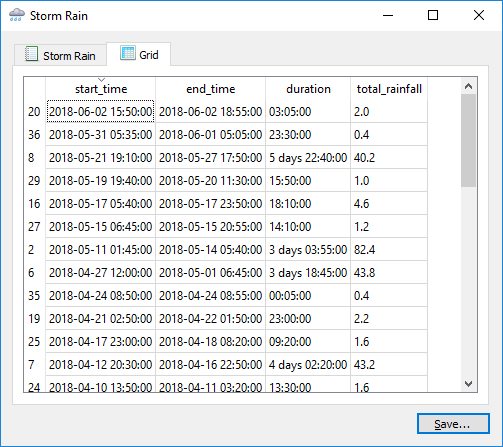
\includegraphics[scale=0.5]{images/table_output}
 \caption{Table Output View}
 \label{img_table_output}
\end {figure}

A table output definition looks like the following where the \verb|query| property specifies the query to display or save:
\begin{lstlisting}[language=json]
{
	"format": "table",
	"name": "grid",
	"title": "Grid",
	"icon": "../../icons/table",
	"query": "storm_rain",
	"filename": "storm_rain.csv",
	"view_columns": null,
	"save_columns": null        
}
\end{lstlisting}
If the output is the result of a dataset generated by JavaScript the output definition looks much the same but instead of specifying a query name, specify the generated dataset name:
\begin{lstlisting}[language=json]
{
	"format": "table",
	"name": "grid",
	"title": "Grid",
	"icon": "../../icons/table",
	"dataset": "daily_sunshine_hours",
	"filename": "daily_sunshine_hours.csv",
	"view_columns": null,
	"save_columns": null        
}
\end{lstlisting}


The \verb|view_columns| and \verb|save_columns| properties allow for renaming columns in both the GUI table view (figure \ref{img_table_output}) as well as CSV file output (when the reports output type is \verb|save| or the user clicks the save button) respectively. These properties take an object mapping SQL column names to their display names:
\begin{lstlisting}[language=json]
{
	"start_time": "Start Time",
	"end_time": "End Time",
	"duration": "Duration",
	"total_rainfall": "Total Rainfall"        
}
\end{lstlisting}

The object only needs to include columns to be renamed - any columns not included in the object will appear using the SQL column name instead. To hide a column entirely from either the table view or CSV output, set its name to null. For example, the following would hide the \verb|start_time| and \verb|end_time| columns in the output in figure \ref{img_table_output} while leaving \verb|duration| and \verb|total_rainfall| named after the SQL column names:
\begin{lstlisting}[language=json]
{
	"start_time": null,
	"end_time": null
}
\end{lstlisting}


\section{HTML  and Text Outputs}
HTML outputs can show formatted text (figure \ref{img_html_output}) using a limited HTML subset (described in appendix \ref{app_html_subset}). If the reports output type is \verb|save| rather than \verb|show| then there are no limitations on the HTML output that can be produced.

\begin {figure}[!ht]
 \centering
 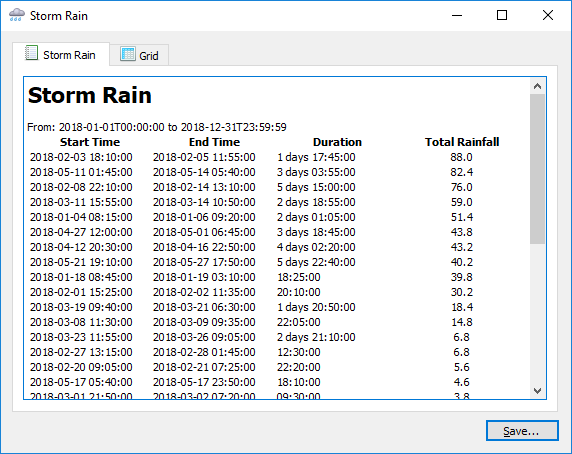
\includegraphics[scale=0.5]{images/html_output}
 \caption{HTML Output View}
 \label{img_html_output}
\end {figure}

Plain text outputs can generate and display plain text documents (figure \ref{img_text_output}) which are shown to the user with a fixed with font with word wrap turned off by default to preserve formatting. If the output type is \verb|save| rather than \verb|show| this output format could be used to generate other document formats. 

\begin {figure}[!ht]
 \centering
 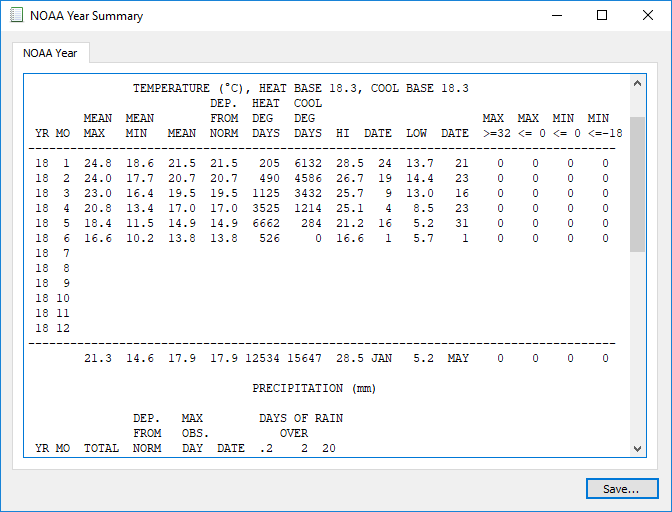
\includegraphics[scale=0.5]{images/text_output}
 \caption{Plain Text Output View}
 \label{img_text_output}
\end {figure}

Both HTML and text outputs are generated using mustache templates. See the mustache manual for writing these templates: \url{https://mustache.github.io/mustache.5.html}. 

An HTML or text output definition looks like:
\begin{lstlisting}[language=json]
 {
	"name": "html",
	"title": "Sun",
	"icon": "../../icons/report",
	"format": "html",
	"template": "sun.html",
	"view_template", "view_sun.html",
	"filename": "sun.html"
},
\end{lstlisting}

Where the \verb|format| parameter is either \verb|html| for html output or \verb|text| for plain text output. If word wrapping is suitable for the report it can be enabled by using the format parameter \verb|text_wrapped| instead; this has no affect when the report is saved.

The \verb|template| parameter specifies the mustache template to produce output with. 

The optional \verb|view_template| parameter specifies an additional template for producing the on-screen view of the report. When this parameter is supplied, the \verb|template| parameter will be used to produce output for saving. This allows saved versions of HTML reports to use more advanced formatting than that allowed by appendix \ref{app_html_subset}.

\subsection{Template Parameters}
All query parameters are available as template parametes. For example:
\begin{verbatim}
Station Code: {{stationCode}}
Time span: {{start}} - {{end}}
\end{verbatim}

This includes any additional parameters from the reports custom criteria page (if it has one).

Each query executed is also available as a list parameter. For example, the following query named \verb|temperatures| and the following HTML template could be used to list temperatures within the reports timespan:
\begin{lstlisting}[language=SQL]
select
 s.time_stamp,
 s.temperature
from sample s
inner join station stn on stn.station_id = s.station_id
where stn.code = (:stationCode)::varchar(5)
and s.time_stamp between :start and :end;
\end{lstlisting}

\begin{lstlisting}[language=HTML]
<html><body>
<table>
<tr><th>Time</th><th>Temperature</th></tr>
{{#temperatures}}
<tr><td>{{time_stamp}}</td><td>{{temperature}}</td></tr>
{{/temperatures}}
</body></html>
\end{lstlisting}

\subsection{Template Partials}
Template partials can be placed in the \verb|partials| subdirectory and must have the \verb|.mustache| file extension. They can then be included in templates via \verb|{{>partial_name}}|.

\subsection{Chart and Data  Links}
The Report Display Window supports links that open a new chart in the Chart Window or show data in the View Data window. Links for a chart start with \verb|zxw://plot| while links to show data start with \verb|zxw://view-data|. Details about the timespan and columns or graphs to include (along with a title for charts) are supplied via query string parameters.

Required parameters are:

\begin{tabular}{p{3.5cm} p{2.5cm} p{7.6cm}}
\hline
\textbf{Parameter} & \textbf{Type} & \textbf{Description} \\
\hline
\verb|start| & ISO8601 Time & Start time for the chart \\
\verb|end| & ISO8601 Time & End time for the chart \\
\verb|graphs| or \verb|columns|& string & List of graphs (or columns for the view data window) to include.\\
\hline
\end{tabular}

Where \verb|graphs| or \verb|columns| is a list of graphs separated by the \verb|+| character. For example, \verb|rainfall+humidity|. The standard graphs or columns that can be included are:
\begin{itemize}
\item \verb|temperature|
\item \verb|indoor_temperature|
\item \verb|apparent_temperature|
\item \verb|wind_chill|
\item \verb|dew_point|
\item \verb|humidity|
\item \verb|indoor_humidity|
\item \verb|pressure|
\item \verb|rainfall|
\item \verb|average_wind_speed|
\item \verb|gust_wind_speed|
\item \verb|wind_direction|
\item \verb|time| (included by default for graphs but not for the view data window)
\end{itemize}

For davis stations, the following extra graphs are available:
\begin{itemize}
\item \verb|solar_radiation|
\item \verb|uv_index|        
\item \verb|reception|
\item \verb|high_temperature|
\item \verb|low_temperature|
\item \verb|high_rain_rate|      
\item \verb|gust_wind_speed|
\item \verb|evapotranspiration|  
\item \verb|high_solar_radiation|
\item \verb|high_uv_index|
\end{itemize}
The solar radiation, UV index and evapotranspiration graphs are specific to the Vantage Pro2 Plus while the reception grpah is specific to wireless stations.

Optional parameters are:

\begin{tabular}{p{2.5cm} p{2.5cm} l}
\hline
\textbf{Parameter} & \textbf{Type} & \textbf{Description} \\
\hline
\verb|title| & string & Chart title \\
\verb|aggregate| & string & Aggregate Function \\
\verb|grouping| & string & Aggregate Group Size \\
\verb|group_minutes| & integer & Group size in minutes \\
\hline
\end{tabular}

Where the value for \verb|aggregate| can be one of:

\begin{itemize}
\item \verb|none| - no aggregate
\item \verb|average|
\item \verb|min|
\item \verb|max|
\item \verb|sum| - only useful for rainfall
\item \verb|running_total| - only useful for rainfall
\end{itemize}

If an aggregate is supplied then the \verb|grouping| must be specified. This can be one of:

\begin{itemize}
\item \verb|hour|
\item \verb|day|
\item \verb|month|
\item \verb|year|
\item \verb|custom|
\end{itemize}

If the grouping is \verb|custom| then the \verb|group_minutes| parameter must be supplied specifying the number of minutes to group by.

\subsubsection{Example}
The following produces a chart titled "Storm Starting start-time" including a single rainfall graph using the running total aggregate. The group size is set to 5 minutes.
\begin{verbatim}
zxw://plot?start={{start_time}}&end={{end_time}}
        &title=Storm Starting {{start_time}}&graphs=rainfall
        &aggregate=running_total&grouping=custom&group_minutes=5
\end{verbatim}

And this will show the same set of data in the view data window:
\begin{verbatim}
zxw://view-data?start={{start_time}}&end={{end_time}}
        &graphs=time+rainfall&aggregate=running_total
        &grouping=custom&group_minutes=5
\end{verbatim}


\subsection{Links to the View Images window}
Links to the View Images window are also supported. These start with \verb|zxw://view-images|.

Required parameters are:

\begin{tabular}{p{3.5cm} p{2.5cm} p{7.6cm}}
\hline
\textbf{Parameter} & \textbf{Type} & \textbf{Description} \\
\hline
\verb|date| & ISO8601 date & Date to expand in the images window \\
\hline
\end{tabular}

\subsubsection{Example}
The following opens the view images window and expands the 2019, August, 10th nodes to show images for the 10th of August 2019:
\begin{verbatim}
zxw://view-images?date=2019-08-10
\end{verbatim}


\chapter{Custom Criteria Pages}
Custom Criteria Pages allow collecting additional report parameters using a custom UI component. These consist of a single Qt Designer \verb|.ui| file which is displayed to the user after the time span page. Any supported input widgets are turned into parameters which are available to both queries and output templates. The widgets Object Name is used as the name of the parameter.

To create a UI file to use as a Custom Criteria Page, use Qt Designer 4.8 to create a new form of type Widget (figure \ref{img_new_widget}). Then add its filename to the Report Definition:

\begin{lstlisting}[language=json]
{
    "criteria_ui": "foo.ui"
}
\end{lstlisting}

\begin {figure}[!ht]
 \centering
 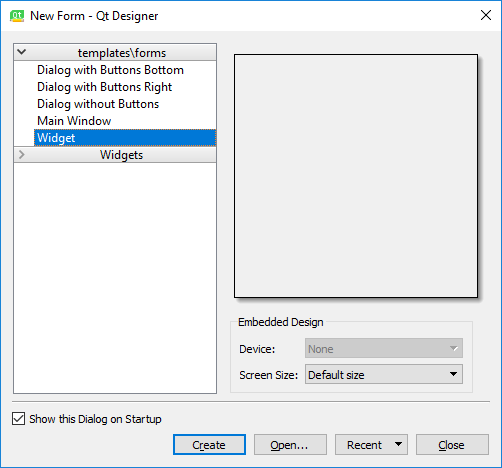
\includegraphics[scale=0.5]{images/new_widget}
 \caption{New Widget}
 \label{img_new_widget}
\end {figure}

The following input widgets are supported:
\begin{itemize}
\item QLineEdit
\item QComboBox
\item QTextEdit
\item QPlainTextEdit
\item QSpinBox
\item QDoubleSpinBox
\item QTimeEdit
\item QDateEdit
\item QDateTimeEdit
\item QDial
\item QSlider
\item QRadioButton
\item QCheckBox
\item QGroupBox (when checkable)
\item QLabel (for display only)
\end{itemize}

Any input entered into the above widgets is saved automatically for the current weather station. Next time the report is run the criteria page will have the previously used values loaded.

Any other  widgets can be used in the UI for display and layout purposes.

The following object names are special:
\begin{itemize}
\item latitude
\item longitude
\item altitude
\item title
\item description
\end{itemize}
When the weather stations configuration provides one of these values any widget with the same name will have its value set to the value the station configuration provides. Any different value entered by the user will not be saved for next time - the form will always start out with the value from the station configuration. The exception to this rule is altitude - if the stations altitude is 0m then any other value entered by the user will be remembered for next time.

Additionally, any widgets called reportName or reportNameBig will have their value set to the title of the report. The reportNameBig widget will be assigned the report name wrapped in \verb|<h1>| HTML tags. The use-case for this is to allow a custom criteria page to have the report name at the top in matching size and location as on the report timespan page.

Any widgets with one of the following names will be automatically populated with time information from the report timespan page:
\begin{itemize}
\item start
\item end
\item year
\item month
\item date
\end{itemize}
Where start and end are datetime values, year is an integer, month and date are dates. These values are suitable for use in QDateEdit, QSpinBox and QDate widgets respectively.

\section{Input Widgets}
\subsection{QLineEdit}
Produces a text parameter.

\begin {figure}[!ht]
 \centering
 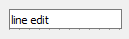
\includegraphics[scale=1.0]{images/widget/qlineedit}
 \caption{QLineEdit}
\end {figure}

\subsection{QComboBox}
Allows the user to choose from a list of options. It produces two parameters - a text parameter containing the text of the currently selected items and an integer parameter containing the index of the currently selected item.

The text parameters name is the object name of the widget while the integer parameter is the object name of the widget with \verb|_id| appended (eg, \verb|foowidget_id|).

\begin {figure}[!ht]
 \centering
 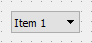
\includegraphics[scale=1.0]{images/widget/qcombobox}
 \caption{QComboBox}
\end {figure}

\subsubsection{Sensor combo box}
You can have zxweather populate a QComboBox with a list of available sensors of different types by adding a string-type dynamic property called \verb|options| to the widget and setting its value to one of the following:

\begin{tabular}{p{5cm} p{8cm} l}
\hline
\textbf{value} & \textbf{Description} \\
\hline
\verb|temperature-sensors| & All available temperature sensors \\
\verb|humidity-sensors| & All available humidity sensors \\
\verb|leaf-wetness-sensors| & Available leaf wetness sensors \\
\verb|leaf-temperature-sensors| & Available leaf temperature sensors only\\
\verb|soil-moisture-sensors| & Available soil moisture sensors\\
\verb|soil-temperature-sensors| & Available soil temperature sensors only\\
\hline
\end{tabular}

\begin {figure}[!ht]
 \centering
 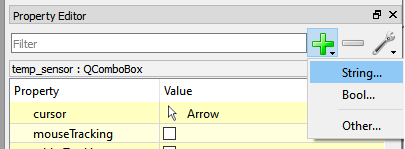
\includegraphics[scale=1.0]{images/add_dynamic_property}
 \caption{Adding a dynamic property in Qt Designer}
\end {figure}

\begin {figure}[!ht]
 \centering
 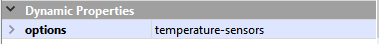
\includegraphics[scale=1.0]{images/dynamic_property}
 \caption{Editing a dynamic property in Qt Designer}
\end {figure}

Where the user has renamed a sensor the sensor will be shown under the users chosen name rather than the system name. The ID produced by these combo boxes is not particuarly useful (as it will depend on what sensors happen to be configured) so these combo boxes produce a third parameter (ending with \verb|_value|) which contains the system name for the chosen sensor. System names for sensors are:
\begin{itemize}
\item \verb|outdoor_temperature|
\item \verb|indoor_temperautre|
\item \verb|outdoor_humidity|
\item \verb|indoor_humidity|
\item \verb|extra_humidity_1|, \verb|extra_humidity_2|
\item \verb|extra_temperature_1|, \verb|extra_temperature_2|, \verb|extra_temperature_3|
\item \verb|leaf_temperature_1|, \verb|leaf_temperature_2|
\item \verb|leaf_wetness_1|, \verb|leaf_wetness_2|
\item \verb|soil_moisture_1|, \verb|soil_moisture_2|, \verb|soil_moisture_3|, \verb|soil_moisture_4|
\item \verb|soil_temperature_1|, \verb|soil_temperature_2|, \verb|soil_temperature_3|, \verb|soil_temperature_4|
\end{itemize}


\subsection{QTextEdit}
A Multi-line text editor that supports pasting of formatted text. Produces HTML output.

\begin {figure}[!ht]
 \centering
 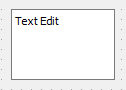
\includegraphics[scale=1.0]{images/widget/qtextedit}
 \caption{QTextEdit}
\end {figure}

\subsection{QPlainTextEdit}

A Multi-line text editor that supports plain text input only.

\begin {figure}[!ht]
 \centering
 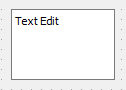
\includegraphics[scale=1.0]{images/widget/qtextedit}
 \caption{QPlainTextEdit}
\end {figure}

\subsection{QSpinBox}

Allows entry of a integer.

\begin {figure}[!ht]
 \centering
 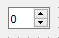
\includegraphics[scale=1.0]{images/widget/qspinbox}
 \caption{QSpinBox}
\end {figure}


\subsection{QDoubleSpinBox}
Allows entry of a floating point number

\begin {figure}[!ht]
 \centering
 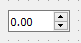
\includegraphics[scale=1.0]{images/widget/qdoublespinbox}
 \caption{QDoubleSpinBox}
\end {figure}

\subsection{QTimeEdit}

Allows entry of time without a date component. It produces a time parameter type.

\begin {figure}[!ht]
 \centering
 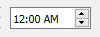
\includegraphics[scale=1.0]{images/widget/qtimeedit}
 \caption{QTimeEdit}
\end {figure}

\subsection{QDateEdit}

Allows entry of a date. It produces a date parameter type.

\begin {figure}[!ht]
 \centering
 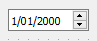
\includegraphics[scale=1.0]{images/widget/qdateedit}
 \caption{QDateEdit}
\end {figure}


\subsection{QDateTimeEdit}

Allows entry of a time and date. It produces a timestamp parameter type.

\begin {figure}[!ht]
 \centering
 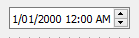
\includegraphics[scale=1.0]{images/widget/qdatetimeedit}
 \caption{QDateTime}
\end {figure}

\subsection{QDial}
A slider shaped like a dial, this widget produces an integer parameter

\begin {figure}[!ht]
 \centering
 
\includegraphics[scale=1.0]{images/widget/qdial}
 \caption{QDial}
\end {figure}

\subsection{QSlider}

This widget is available in both vertical and horizontal orientations with and without notches. It produces an integer parameter.

\begin {figure}[!ht]
 \centering
 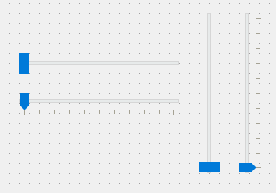
\includegraphics[scale=1.0]{images/widget/qslider}
 \caption{QSlider}
\end {figure}

\subsection{QRadioButton}

These widgets allow the user to choose between a number of mutually exclusive options. Each widget produces a boolean parameter with only the currently selected radio button having its parameter set to true.

\begin {figure}[!ht]
 \centering
 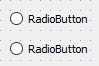
\includegraphics[scale=1.0]{images/widget/qradiobutton}
 \caption{QRadioButton}
\end {figure}

\subsection{QCheckBox}

This widget produces a boolean parameter.

\begin {figure}[!ht]
 \centering
 
\includegraphics[scale=1.0]{images/widget/qcheckbox}
 \caption{QCheckBox}
\end {figure}

\subsection{QGroupBox}

Group boxes are used for grouping togeter widgets. When a group box is made checkable it produces a boolean parameter.

\begin {figure}[!ht]
 \centering
 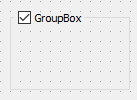
\includegraphics[scale=1.0]{images/widget/qgroupbox}
 \caption{QGroupBox}
\end {figure}



%%%%%%%%%%%%%%%%%%%%%%%%%%%%%%%%%%%%%%%%%%%%%%%%%%%%%%%%%%%%%%%%%%%%%%%%%%%%%
% Appendix
%%%%%%%%%%%%%%%%%%%%%%%%%%%%%%%%%%%%%%%%%%%%%%%%%%%%%%%%%%%%%%%%%%%%%%%%%%%%%
\appendix

\chapter{SQLite Cache Database Schema}
The SQLite Cache Database is used to store downloaded weather data for plotting charts, showing and exporting data and running reports. When a report is run with the \emph{Web Interface} Sample Data Source the first step of running the report is ensuring all required data exists in this database before running the report.

This appendix describes the tables in that database.

\section{data\_file Table}
This table lists data files that were downloaded from the Web Interface to supply data in the sample table.

\begin{tabular}{p{2.5cm} p{2.5cm} l}
\hline
\textbf{Column} & \textbf{Type} & \textbf{Description} \\
\hline
\verb|id| & integer & Primary Key\\
\verb|station| & integer & Foreign Key to Station table\\
\verb|url| & text & URL for this data file. Unique.\\
\verb|last_modified| & integer & Last modified time for the URL in UNIX Time\\
\verb|size| & integer & Size of the data file in bytes\\
\hline
\end{tabular}

\section{db\_metadata Table}
This table contains metadata about the database. This is stored as a set of key/value associations.

\begin{tabular}{p{2.5cm} p{2.5cm} l}
\hline
\textbf{Column} & \textbf{Type} & \textbf{Description} \\
\hline
\verb|k| & text & Primary Key\\
\verb|v| & text & Value\\
\hline
\end{tabular}

Standard keys are:

\begin{tabular}{p{2.5cm} l}
\hline
\textbf{Column} & \textbf{Description} \\
\hline
\verb|v| & Database schema version. Value is 2 for zxweather 1.0.0\\
\hline
\end{tabular}

\section{image Table}
Stores information about downloaded images.

\begin{tabular}{p{2.5cm} p{2.5cm} l}
\hline
\textbf{Column} & \textbf{Type} & \textbf{Description} \\
\hline
\verb|id| & integer & Primary Key\\
\verb|image_set| & integer & Foreign Key to \verb|image_set| table.\\
\verb|source| & integer & Foreign Key to \verb|image_source| table.\\
\verb|timestamp| & integer & Time of the image in UNIX Time format.\\
\verb|date| & text & Image date.\\
\verb|type_code| & text & Image type code.\\
\verb|type_name| & text & Image type name.\\
\verb|title| & text & Image type \\
\verb|description| & text & Image description\\
\verb|mime_type| & text & Image mime type\\
\verb|url| & text & Original URL on the Web Interface for the image\\
\verb|metadata| & text & JSON document containing metadata for the image\\
\verb|meta_url| & text & Original URL on the Web Interface for the metadata\\
\hline
\end{tabular}

\section{image\_dates Table}
For each image source this table has a list of dates that have images available. This is primarily for reports that need to generate links to the view images window. Any date in this table should be valid for the view images window.

\begin{tabular}{p{2.5cm} p{2.5cm} p{8.6cm}}
\hline
\textbf{Column} & \textbf{Type} & \textbf{Description} \\
\hline
\verb|image_source_id| & integer & ID of an image source in the \verb|image_source| table.\\
\verb|date| & text & An ISO8601 date for which there are images available for the image source \\
\hline
\end{tabular}

\section{image\_set Table}
This is the equivalent of the \verb|data_file| table but for images. It records the JSON index file that supplied information about the images. Images that were downloaded due to new image notifications via the live data system are stored against a temporary image set. The URL for temporary image sets consists of the stations URL prefixed with \verb|::temporary_image_set:|.


\begin{tabular}{p{2.5cm} p{2.5cm} p{8.6cm}}
\hline
\textbf{Column} & \textbf{Type} & \textbf{Description} \\
\hline
\verb|id| & integer & Primary Key\\
\verb|image_source| & integer & Image source the image came from\\
\verb|url| & text & URL for the image index file\\
\verb|last_modified| & integer & Last modified timestamp for the index file in UNIX time.\\
\verb|size| & integer & Size of the image index file in bytes.\\
\verb|is_valid| & integer & If the index is valid and doesn't need redownloading\\
\hline
\end{tabular}

\section{image\_source Table}
Stores information about an image source (camera, satellite receiver, etc).

\begin{tabular}{p{2.5cm} p{2.5cm} l}
\hline
\textbf{Column} & \textbf{Type} & \textbf{Description} \\
\hline
\verb|id| & integer & Primary key\\
\verb|station| & integer & Foreign Key to the Station table\\
\verb|code| & text & Image Source code\\
\verb|name| & text & Name of the Image Source\\
\verb|description| & text & Description of the Image Source\\
\hline
\end{tabular}

\section{sample Table}
This table stores weather data downloaded from the Web Interface. Each row is linked back to the original data file that provided it in addition to the station it belongs to. It is ued by the desktop client for plotting charts, viewing and exporting data as well as running reports.

Column names in this table match those of the PostgreSQL schema where possible to ease porting queries. A number of columns in this table would, in the PostgreSQL schema, normally live in other tables. To ease porting of queries compatibility views for some of these tables are provided.

\begin{tabular}{p{4.7cm} p{1.5cm} l}
\hline
\textbf{Column} & \textbf{Type} & \textbf{Description} \\
\hline
\verb|sample_id| & integer & Primary key\\
\verb|time_stamp| & integer & Time stamp in UNIX Time\\
\verb|indoor_relative_humidity| & integer & Indoor humidity\\
\verb|indoor_temperature| & real & Indoor Temperature in \degree C\\
\verb|relative_humidity|& integer & Outdoor humidity\\
\verb|temperature| & integer & Outdoor temperature in \degree C\\
\verb|dew_point| & real & Dew point in \degree C\\
\verb|wind_chill| & real & Wind chill in \degree C\\
\verb|apparent_temperature| & real & Apparent temperature in \degree C\\
\verb|absolute_pressure| & real & Barometric pressure in hPa. \\
\verb|average_wind_speed| & real & Wind speed over the sample period in m/s\\
\verb|gust_wind_speed| & real & Max wind speed over the sample period in m/s\\
\verb|wind_direction| & integer & Average wind direction over in degrees\\
\verb|rainfall| & real & total rainfall in mm\\
\verb|station_id| & integer & Foreign Key to the station table\\
\verb|solar_radiation| & real & (DS) Solar Radiation in $W/m^2$\\
\verb|uv_index| & real & (DS) UV Index\\
\verb|reception| & real & (DS) Wireless reception quality (precentage)\\
\verb|high_temperature| & real & (DS) Max temperature in \degree C\\
\verb|low_temperature| & real & (DS) Min temperature in \degree C\\
\verb|high_rain_rate| & real & (DS) Max rain rate in mm/h\\
\verb|gust_wind_direction| & integer & (DS) Direction of the wind gust in degrees\\
\verb|evapotranspiration| & real & (DS) Total Evapotranspiration\\
\verb|high_solar_radiation| & real & (DS) Max solar radiation over in $W/m^2$\\
\verb|high_uv_index| & real & (DS) High UV Index over the sample period\\
\verb|forecast_rule_id| & integer & (DS) Forecast rule ID\\
\verb|data_file| & integer & Foreign Key to the \verb|data_file| table\\
\hline
\end{tabular}

The columns marked (DS) are only populated for Davis weather stations (Vantage Pro2, Pro2 Plus and Vue). The Solar Radiation, UV Index and Evapotranspiration columns are only populated when the weather station is fitted with solar sensors (a Vantage Pro2 Plus or a Vantage Vue receiving data from a Vantage Pro2 Plus ISS). These values live in the \verb|davis_sample| table in the PostgreSQL schema and are available from a view of the same name in this database to ease porting.

Note that in this table the \verb|absolute_pressure| column may in fact contain sea level pressure depending on the type of the associated weather station.

\section{davis\_sample View}
This view is provided for compatibility with the PostgreSQL schema. Its contents matches that of the \verb|davis_sample| table where data from Davis weather stations is stored.

\begin{tabular}{p{4.7cm} p{1.5cm} l}
\hline
\textbf{Column} & \textbf{Type} & \textbf{Description} \\
\hline
\verb|sample_id| & integer & Primary key\\
\verb|high_temperature| & real & Max temperature in \degree C\\
\verb|low_temperature| & real & Min temperature in \degree C\\
\verb|high_rain_rate| & real & Max rain rate in mm/h\\
\verb|solar_radiation| & real & Solar Radiation in $W/m^2$\\
\verb|wind_sample_count| & integer & Number of wind samples received\\
\verb|gust_wind_direction| & integer & Direction of the wind gust in degrees\\
\verb|average_uv_index| & real & UV Index\\
\verb|evapotranspiration| & real & Total Evapotranspiration\\
\verb|high_solar_radiation| & real & Max solar radiation over in $W/m^2$\\
\verb|high_uv_index| & real & High UV Index over the sample period\\
\verb|forecast_rule_id| & integer & Forecast rule ID\\
\hline
\end{tabular}

The \verb|wind_sample_count| value is derived from the reception column in the sample table based on the stations broadcast Id. This is just a reversal of the formula originally used to calculate the reception.

\section{station Table}
Stores information about a weather station. Its structure is similar to that of the station table in the PostgreSQL schema to ease porting of queries.

\begin{tabular}{p{3.5cm} p{1.3cm} l}
\hline
\textbf{Column} & \textbf{Type} & \textbf{Description} \\
\hline
\verb|station_id| & integer & Primary Key\\
\verb|code| & text & URL for the weather station  \\
\verb|title| & text & Weather station title\\
\verb|description| & text & Description of the weather station\\
\verb|station_type_id| & integer & Foreign Key to the \verb|station_type| table\\
\verb|sample_interval| & integer & Sample interval in minutes\\
\verb|latitude| & real & Latitude\\
\verb|longitude| & real & Longitude\\
\verb|altitude| & real & Altitude in meters\\
\verb|solar_available| & boolean & True if Solar data is available in the sample table\\
\verb|davis_broadcast_id| & integer & Davis stations - Wireless broadcast ID\\
\hline
\end{tabular}

The \verb|solar_available| column will be set for Vantage Pro2 Plus stations (and Vue stations receiving from a Vantage Pro2 Plus ISS). It means that the Solar Radiation, UV Index and Evapotranspiration columns are set.

\section{station\_type Table}
\begin{tabular}{p{3cm} p{2.5cm} l}
\hline
\textbf{Column} & \textbf{Type} & \textbf{Description} \\
\hline
\verb|station_type_id| & integer & Primary Key\\
\verb|code| & text & Station type code\\
\verb|title| & text & Station type name\\
\hline
\end{tabular}




\chapter{HTML Subset for Display}
\label{app_html_subset}
Only a limited subset of HTML is supported for display within the reporting system. This appendix describes the elements and attributes available.

\section{Elements}
\begin{tabular}{p{3cm} p{10.6cm}}
\hline
\textbf{Element} & \textbf{Comments} \\
\hline
\verb|a| & Supports \verb|href| and \verb|name| attributes\\
\verb|address| &\\
\verb|b|&\\
\verb|big|&\\
\verb|blockquote|&\\
\verb|body|& supports the \verb|bgcolor| attribute\\
\verb|br|&\\
\verb|center|&\\
\verb|cite|& same as \verb|i|\\
\verb|code|& same as \verb|tt|\\
\verb|dd|&\\
\verb|dfn|& same as \verb|i|\\
\verb|div| & Supports standard block attributes\\
\verb|dl| & Supports standard block attributes\\
\verb|dt| & Supports standard block attributes\\
\verb|em| & Same as \verb|i|\\
\verb|font| & Supports \verb|size|, \verb|face| and \verb|color| attributes\\
\verb|h1| & Supports standard block attributes\\
\verb|h2| & Supports standard block attributes\\
\verb|h3| & Supports standard block attributes\\
\verb|h4| & Supports standard block attributes\\
\verb|h5| & Supports standard block attributes\\
\verb|h6| & Supports standard block attributes\\
\verb|head|&\\
\verb|hr|&Supports \verb|width| attribute as absolute or relative value\\
\verb|html| &\\
\verb|i| &\\
\verb|img| & Supports \verb|src|, \verb|width| and \verb|height| attributes\\
\verb|kbd| &\\
%\verb|meta| & \\
\hline
\end{tabular}

\begin{tabular}{p{3cm} p{10.6cm}}
\hline
\textbf{Element} & \textbf{Comments} \\
\hline
\verb|li| & \\
\verb|nobr| & \\
\verb|ol| & Supports standard list attributes\\
\verb|p| & Supports standard block attributes\\
\verb|pre| &\\
\verb|s| & \\
\verb|samp| & \\
\verb|small| & \\
\verb|span| & \\
\verb|strong| & same as \verb|b|\\
\verb|style| & Supports a limited subset of CSS\\
\verb|sub| &\\
\verb|sup| &\\
\verb|table| & supports \verb|border|, \verb|bgcolor|, \verb|cellspacing|, \verb|cellpadding|, \verb|width| (absolute or relative) and \verb|height|\\
\verb|tbody| & does nothing\\
\verb|td| & Supports standard table cell attributes\\
\verb|tfoot| & does nothing\\
\verb|th| & Supports standard table cell attributes\\
\verb|thead| & Used when printing tables that span multiple pages\\
\verb|title| & \\
\verb|tr| & supports the \verb|bgcolor| attribute\\
\verb|tt| & \\
\verb|u| & \\
\verb|ul| & Supports standard list attributes\\
\verb|var| & Same as \verb|i|\\
\hline
\end{tabular}

\section{Block Attributes}
The following attributes are supported by the \verb|div|, \verb|dl|, \verb|dt|, \verb|h1|, \verb|h2|, \verb|h3|, \verb|h4|, \verb|h5|, \verb|h6|, \verb|p| tags:
\begin{itemize}
\item \verb|align| (\verb|left|, \verb|right|, \verb|center|, \verb|justify|)
\item \verb|dir| (\verb|ltr|, \verb|rtl|)
\end{itemize}

\section{List Attributes}
The following attributes are supported by the \verb|ol| and \verb|ul| tags:
\begin{itemize}
\item \verb|type| (\verb|1|, \verb|a|, \verb|A|, \verb|square|, \verb|disc|, \verb|circle|)
\end{itemize}

\section{Table Cell Attributes}
The following attributes are supported by the \verb|td| and \verb|th| tags:
\begin{itemize}
\item \verb|width| (absolute, relative or none)
\item \verb|bgcolor|
\item \verb|colspan|
\item \verb|rowspan|
\item \verb|align| (\verb|left|, \verb|right|, \verb|center|, \verb|justify|)
\item \verb|valign| (\verb|top|, \verb|middle|, \verb|bottom|)
\end{itemize}

\section{CSS Properties}
The following CSS Properties are supported

\begin{tabular}{p{3.1cm} p{6cm} p{4.5cm}}
\hline
\textbf{Property} & \textbf{Values} & \textbf{Comments} \\
\hline
\verb|background-color| & <color> & element background colour \\
\verb|background-image| & <uri> & element background imaage \\
\verb|color| & <color> & Text colour \\
\verb|font-family| & <family name> & \\
\verb|font-size| & [ small | medium | large | x-large | xx-large ] | <size>pt | <size>px & Font size relative to the document font or fixed size \\
\verb|font-style| & [ normal | italic | oblique] & \\
\verb|font-weight| & [ normal | bold | 100 | 200 | 300 | 400 | 500 | 600 | 700 | 800 | 900 ] & \\
\verb|text-decoration| & none | [underline || overline || line-through] & \\
\verb|font| & [[<font-style> || <font-weight>]? <font-size> <font-family>] & \\
\verb|text-indent| & <length>px & First line text indent in pixels\\
\verb|white-space| & normal | pre | nowrap | pre-wrap| & \\
\verb|margin-top| & <length>px & \\
\verb|margin-bottom| & <length>px & \\
\verb|margin-left| & <length>px & \\
\verb|margin-right| & <length>px & \\
\verb|padding-top| & <length>px & \\
\verb|padding-bottom| & <length>px & \\
\verb|padding-left| & <length>px & \\
\verb|padding-right| & <length>px & \\
\verb|padding| & <length>px & Short-hand for setting all sides at once\\
\verb|vertical-align| & baseline | sub | super | middle | top | bottom & \\
\verb|border-color| & <color> & For text tables\\

\verb|border-style| & none | dotted | dashed | dot-dash | dot-dot-dash | solid | double | groove | ridge | inset | outset & \\
\verb|background| & [<background-color> || <background-image>] & background shorthand\\
\hline
\end{tabular}

\begin{tabular}{p{3.1cm} p{6cm} p{4.5cm}}
\hline
\textbf{Property} & \textbf{Values} & \textbf{Comments} \\
\hline

\verb|pre-break-before| & [ auto | always ] & \\
\verb|pre-break-after| & [ auto | always ] & \\
\verb|float| & [ left | right | none ] & Only supported for tables and images \\
\verb|text-transform| & [ uppercase | lowercase ] & \\
\verb|font-variant| & small-caps & \\
\verb|word-spacing| & <width>px & \\
\hline
\end{tabular}

\subsection{CSS Selectors}
All CSS 2.1 selector classes are supported except pseudo-class selectors like \verb|:first-child|, \verb|:visited|, etc.



\chapter{Built-in Reports}
\label{app_built_in_reports}
The zxweather Desktop Client implements a number of common reports which aim to produce output compatible with existing software such as WeatherLink where feasible in addition to its own unique reports. Built-in reports consist of the following:
\begin{itemize}
\item Leaf Wet Hours
\item Monthly Averages
\item NOAA Month Summary
\item NOAA Year Summary
\item Rainfall
\item Soil Temperature Hours
\item Station Records
\item Storm Rain
\item Sun
\item Sunshine hours
\end{itemize}

Some of these reports require sensors not available on all weather stations (eg, Solar Radiation) or sensors that are optional extras (eg, Leaf Wetness). When a required sensor is missing the report will not be available.

All of these reports are built using the capabilities described in this manual - anything these reports can do a custom report can do as well. This section describes these reports, how they work and the files that make them up. Any files placed in the report search path with conflicting names will replace the built-in report files allowing them to be customised.

\section{Leaf Wet Hours}
This report calculates total leaf wet hours for a chosen date range plus a daily total for each day in that date range. It is only available for stations equipped with at least one Leaf Wetness Sensor. When multiple sensors are present it will calculate for each sensor.

Leaf Wet Hours are calculated using three threshold values:
\begin{itemize}
\item Minimum leaf wetness
\item Minimum temperature
\item Maximum temperature
\end{itemize}

One leaf wet hour will be one hour where the leaf wetness sensor is above the set minimum and the chosen temperature sensors value is between the set minimum and maximum. Any temperature sensor can be chosen for this calculation.

The reports emulates the one shipped with WeatherLinks Ag/Turf module with the following differences:
\begin{itemize}
\item Fix typo in "Leaf Sensor Nunber"
\item Include custom names for the temperature sensor and leaf wetness sensors where they have been set
\item Fix truncation of minimum and maximum temperature values to 0dp (weatherlink does this with no rounding - a value of 4.9 becomes 4.0)
\item Fix incorrect display of minimum and maximum temperatures in report output when using Celsius. In weatherlink an input of 1.0\degree C produces an output of 0.\degree C due to truncation between conversion to Fahrenheit and back to Celsius.
\item Calculation is performed with the temperature thresholds as entered without truncating them to 0dp
\item Fix day count to the number of dates between the reports start date and today if the reports end date is in the future ("Last 30 days" doesn't make sense when the report is really run for this month and we're only 5 days in)
\end{itemize}

These changes will result in slightly different output compared to WeatherLink but the results should be no less accurate.

\subsection{Files}

\begin{tabular}{p{6cm} l}
\hline
\textbf{File} & \textbf{Description} \\
\hline
\verb|libs/moment.js| & Date/time library\\
\verb|libs/moment-timezone-with-data-2012-2022.js| & \\
& Timezone data \\
\verb|partials/summary.mustache| & Template containing per-sensor summary data\\
\verb|criteria.ui| & Report criteria UI \\
\verb|description.html| & Report description.\\
\verb|psql.sql| & Report Query for PostgreSQL. \\
\verb|report.js| & Summary data calculation and output formatting\\
\verb|report.json| & Report Definition. \\
\verb|sqlite.sql| & Report Query for SQLite. \\
\verb|wlformat.txt| & main output template.\\
\hline
\end{tabular}

All files live in a directory named \verb|leaf_wet_hours|.

\section{Monthly Averages}
This report runs over the weather stations entire data set aggregating data by month. It computes the following values:
\begin{itemize}
\item Average High
\item Daily Mean
\item Average Low
\item Average Rain
\item Average Rain days (days where rainfall >= 1.0mm)
\item Average Humidity
\item Average Wind Speed
\item Average Gale Days (days where average wind is >= 63km/h)
\end{itemize}

Its custom criteria page allows choosing between metric and imerial units and between m/s and km/h for metric wind speed.

Output is formatted text (HTML) and CSV.

\subsection{Files}

\begin{tabular}{p{4.5cm} l}
\hline
\textbf{File} & \textbf{Description} \\
\hline
\verb|criteria_pg.sql| & Criteria formatting query for PostgreSQL.\\
\verb|criteria_sqlite.sql| & Criteria formatting query for SQLite.\\
\verb|description.html| & Report description.\\
\verb|postgres.sql| & Report Query for PostgreSQL. \\
\verb|report.json| & Report Definition. \\
\verb|sqlite.sql| & Report Query for SQLite. \\
\verb|template.html| & Output template. \\
\verb|units.ui| & Custom criteria page. \\
\hline
\end{tabular}

All files live in a directory named \verb|averages_report|.

\section{NOAA Month Summary}
This produces the common NOAA Month summary report available in other software packages. This is a plain-text report  summarising a single month from a single year. Its report criteria page includes the following output settings:
\begin{itemize}
\item Station Name, Location, Coordinates and Altitude
\item Heat and cool base (for calculating heating and cooling degree days)
\item Output units
\end{itemize}

\subsection{Output}

 Its output includes the following basic weather station information:
\begin{itemize}
\item Station Name
\item City
\item State
\item Altitude
\item Latitude and Longitude
\end{itemize}

Output per day is:
\begin{itemize}
\item Mean Temperature
\item High Temperature and time of day
\item Low temperature and time of day
\item Heating degree days
\item Cooling degree days
\item Total rainfall
\item Average Wind Speed
\item High wind speed and time of day
\item Dominant wind direction as a compass point
\end{itemize}

The summary row for the entire month contains:
\begin{itemize}
\item Mean temperature
\item High temperature and day of month
\item Low temeprature and day of month
\item Total heating degree days
\item Total cooling degree days
\item Total rainfall
\item Average wind speed
\item High wind speed and day of month
\item Dominant wind direction
\end{itemize}

Additional summary data:
\begin{itemize}
\item Number of days where the high temperature was 32 \degree C or higher.
\item Number of days where the high temperature was 0 \degree C or lower.
\item Number of days where the low temperature is 0 \degree C or lower.
\item Number of days where the low temperature is -18 \degree C or lower.
\item Maximum single-day rain with date
\item Number of days where rain was above 0.2mm, 2mm or 20mm.
\end{itemize}

\subsection{Files}
\begin{tabular}{p{4.5cm} l}
\hline
\textbf{File} & \textbf{Description} \\
\hline
\verb|criteria.ui| & Criteria page. \\
\verb|criteria_psql.sql| & Criteria formatting query for PostgreSQL. \\
\verb|criteria_sql.sql| & Criteria formatting query for SQLite. \\
\verb|daily_psql.sql| & Per-day query for PostgreSQL. \\
\verb|daily_sqlite.sql| & Per-day query for SQLite. \\
\verb|description.html| & Report description. \\
\verb|month_psql.sql| & Per-month query for PostgreSQL. \\
\verb|month_sqlite.sql| & Per-month query for SQLite. \\
\verb|noaamo.txt| & Output template. \\
\verb|report.json| & Report Definition. \\
\hline
\end{tabular}

All files live in a directory named \verb|noaamo|.

\section{NOAA Year Summary}
This produces the common NOAA Year summary report available in other software packages. This is a plain-text report summarising an entire year. Its report criteria page includes the following output settings:
\begin{itemize}
\item Station Name, Location, Coordinates and Altitude
\item Heat and cool base (for calculating heating and cooling degree days)
\item Output units
\item Normal rainfall and mean temperature per month
\end{itemize}

\subsection{Output}

Its output includes the following basic weather station information:
\begin{itemize}
\item Station Name
\item City
\item State
\item Altitude
\item Latitude and Longitude
\end{itemize}

Data is divided into three tables: Temperature, Precipitation and Wind Speed. Data per month is:
\begin{itemize}
\item Mean high temperature
\item Mean low temperature
\item Mean temperature
\item Departure from normal mean temperature
\item Total heating degree days
\item Total cooling degree days
\item High temperature and day of month
\item Low temperature and day of month
\item Number of days where the high termperature was 32 \degree C or higher
\item Number of days where the high temperature was 0 \degree C or lower
\item Number of days where the low temperature was 0 \degree C or lower
\item Number of days where the low temperature was -18 \degree C or lower
\item Total rainfall
\item Departure from normal total rainfall
\item Max observed day rainfall with day of month
\item Number of days over 0.2mm of rain
\item Number of days over 2.0mm of rain
\item Number of days over 20mm of rain
\item Average wind speed
\item High wind speed and day of month
\item Dominant wind direction
\end{itemize}

The summary row for the entire year contains:
\begin{itemize}
\item Mean high temperature
\item Mean low temperature
\item Mean temperature
\item Departure from normal mean temperature
\item Total heating degree days
\item Total cooling degree days
\item High temperature and month containing the high temperature
\item Low temeprature and month containing the high temperature
\item Number of days where the high termperature was 32 \degree C or higher
\item Number of days where the high temperature was 0 \degree C or lower
\item Number of days where the low temperature was 0 \degree C or lower
\item Number of days where the low temperature was -18 \degree C or lower
\item Total rainfall
\item Departure from normal year rainfall
\item Max observed month rainfall and the month that occurred in
\item Number of days over 0.2mm of rain
\item Number of days over 2.0mm of rain
\item Number of days over 20mm of rain
\item Average wind speed
\item High wind speed and the month that occurred in
\item Dominant wind direction
\end{itemize}

\subsection{Files}
\begin{tabular}{p{4.5cm} l}
\hline
\textbf{File} & \textbf{Description} \\
\hline
\verb|criteria.ui| & Criteria page. \\
\verb|criteria_psql.sql| & Criteria formatting query for PostgreSQL. \\
\verb|criteria_sql.sql| & Criteria formatting query for SQLite. \\
\verb|description.html| & Report description. \\
\verb|monthly_psql.sql| & Per-month query for PostgreSQL. \\
\verb|monthly_sqlite.sql| & Permonth query for SQLite. \\
\verb|noaayr.txt| & Output template. \\
\verb|report.json| & Report Definition. \\
\verb|yearly_psql.sql| & Per-year query for PostgreSQL. \\
\verb|yearly_sqlite.sql| & Per-year query for SQLite. \\
\hline
\end{tabular}

\section{Rainfall}
This report calculates rainfall totals by year and month along with per-month highs, lows and averages across the stations entire data set. It does not have a timespan picker or any custom criteria page. The output format is plain text and compatible with the equivalent WeatherLink report.

\subsection{Files}
\begin{tabular}{p{3.8cm} p{10cm}}
\hline
\textbf{File} & \textbf{Description} \\
\hline
\verb|description.html| & Report description. \\
\verb|report.json| & Report Definition.\\
\verb|summary_psql.sql| & PostgreSQL query for computing summary data\\
\verb|summary_sqlite.sql| & SQLite query for computing summary data.\\
\verb|template.txt| & Output template.\\
\verb|yearly_psql.sql| & PostgreSQL query for computing yearly data.\\
\verb|yearly_sqlite.sql| & SQLite query for computing yearly data.\\
\hline
\end{tabular}

\section{Soil Temperature Hours}
This report calculates total soil temperature hours for a chosen date range plus a daily total for each day in that date range. It is best used with a soil moisture probe but is available to be used with any temperature sensor.

One soil temperature hour will be one hour where the temperature sensor is above the set threshold. 

The reports emulates the one shipped with WeatherLinks Ag/Turf module with the following differences:
\begin{itemize}
\item Include custom names for the temperature sensor and leaf wetness sensors where they have been set
\item Fix day count to the number of dates between the reports start date and today if the reports end date is in the future ("Last 30 days" doesn't make sense when the report is really run for this month and we're only 5 days in)
\end{itemize}

These changes will result in slightly different output compared to WeatherLink but the results should be no less accurate.

\subsection{Files}

\begin{tabular}{p{6cm} l}
\hline
\textbf{File} & \textbf{Description} \\
\hline
\verb|libs/moment.js| & Date/time library\\
\verb|libs/moment-timezone-with-data-2012-2022.js| & \\
& Timezone data \\
\verb|criteria.ui| & Report criteria UI \\
\verb|description.html| & Report description.\\
\verb|psql.sql| & Report Query for PostgreSQL. \\
\verb|report.js| & Summary data calculation and output formatting\\
\verb|report.json| & Report Definition. \\
\verb|sqlite.sql| & Report Query for SQLite. \\
\verb|wlformat.txt| & main output template.\\
\hline
\end{tabular}

All files live in a directory named \verb|soil_temp_hours|.

\section{Station Records}
This report finds the highs and lows for the stations entire data set. It produces two HTML format outputs showing the earliest and latest occurrance for each record. It does not have a timespan picker or any custom criteria page.

\subsection{Output}
Each item comes with the date and time of its occurance. This will either be the first time the record occurred or the last time depending on the output.
\begin{itemize}
\item Temperature High and Low
\item Humidity High and Low
\item Wind Chill High and Low
\item Apparent Temperature High and Low
\item Dew Point High and Low
\item Barometer High and Low
\item Average Wind Speed High
\item Gust Wind Speed High
\item Solar Radiation High
\item UV Index High
\item Evapotranspiration High
\item Rain Rate High
\item Total number of rows processed
\end{itemize}

\subsection{Files}
\begin{tabular}{p{4.5cm} l}
\hline
\textbf{File} & \textbf{Description} \\
\hline
\verb|description.html| & Report description. \\
\verb|records.html| & Output template for latest occurrances.\\
\verb|records_early.html| & Output template for earliest occurrances.\\
\verb|records_psql.sql| & PostgreSQL query.\\
\verb|records_sqlite.sql| & SQLite query.\\
\verb|report.json| & Report Definition.\\
\hline
\end{tabular}

\section{Storm Rain}
This report calculates storm rain totals for all storms \emph{starting} within the chosen timespan. All rainfall for these storms is included regardless of whether the rain fell within the chosen timespan or not. This means that some storms may have end dates that fall outside the chosen timespan while other storms with rain in this timespan my be excluded as their start is outside the timespan.

Output is both formatted text (HTML) and CSV (table) consisting of start and end dates, duration and total rainfall.

\subsection{Files}
\begin{tabular}{p{4.5cm} l}
\hline
\textbf{File} & \textbf{Description} \\
\hline
\verb|description.html| & Report description. \\
\verb|postgres.sql| & PostgreSQL query.\\
\verb|report.json| & Report Definition.\\
\verb|sqlite.sql| & SQLite query.\\
\verb|template.html| & HTML output template.\\
\verb|weather-rain.png| & Report Icon.\\
\hline
\end{tabular}

\section{Sun}
This report displays sunrise and sunset times for a chosen timespan.  Its criteria page requires coordinates to calculate times for as well as a timezone.

It produces an HTML output with the folloing data:
\begin{itemize}
\item Date
\item Sunrise and Sunset
\item Day length and difference from previous day
\item Astronomical Twilight Start and End
\item Nautical Twilight Start and End
\item Civil Twilight Start and End
\item Solar noon time
\end{itemize}
The row for today is highlighted. It also contains the coordinates, timespan and timezone

It also produces a plain-text output with:
\begin{itemize}
\item Date
\item Astronomical, Nautical and Civil twilight start
\item Sunrise
\item Sunset
\item Civil, Nautical and Astronomical twilight end
\item Daylight hours
\end{itemize}
This output is compatible with the equivalent report in WeatherLink and includes the coordinates and timezone. Daylight savings mode is always Automatic.



\subsection{Files}
\begin{tabular}{p{3.8cm} p{10cm}}
\hline
\textbf{File} & \textbf{Description} \\
\hline
\verb|libs/moment.js| & Date/time library\\
\verb|libs/moment-timezone-with-data-2012-2022.js| & \\
& Timezone data \\
\verb|criteria.ui| & Report Criteria.\\
\verb|description.html| & Report description. \\
\verb|lat_long.js| & JavaScript code for converting latitude \& longitude to degrees-minutes-seconds format.\\
\verb|report.json| & Report Definition.\\
\verb|solar.js| & Contains the \verb|generate_datasets| function\\
\verb|solar_gen.js| & JavaScript code for calculating sun data.\\
\verb|sun.html| & HTML output template.\\
\verb|weather.png| & Report Icon.\\
\verb|wlformat.txt| & Text output template.\\
\hline
\end{tabular}

\section{Sunshine hours}
This report displays the approximate number of sunshine hours per day based on the calculated theoretical maximum sunshine for the stations coordinates and time of year along with a percentage for the day (sunshine hours out of theoretical maximum). Daily output formats are text (with links to view images for the day where they exist), plain text in the style of WeatherLink, and a sortable grid. Raw per-sample data is also provided in a grid for the first 1000 rows primarily for the purposes of adjusting report parameters to better match actual conditions.

\subsection{Files}
\begin{tabular}{p{3.8cm} p{10cm}}
\hline
\textbf{File} & \textbf{Description} \\
\hline
\verb|libs/moment.js| & Date/time library\\
\verb|libs/moment-timezone-with-data-2012-2022.js| & \\
& Timezone data \\
\verb|criteria.ui| & Report Criteria.\\
\verb|description.html| & Report description. \\
\verb|psql.sql| & PostgreSQL data query.\\
\verb|report.js| & Main data processing script. \\
\verb|report.json| & Report Definition.\\
\verb|solar.js| & astronomical calculations \\
\verb|sqlite.sql| & SQLite data query. \\
\verb|sun_hours.html| & HTML display template.\\
\verb|sun_hours_save.html| & HTML save template.\\
\verb|weather.png| & Report Icon.\\
\verb|wlformat.txt| & Text output template.\\
\hline
\end{tabular}


%%%%%%%%%%%%%%%%%%%%%%%%%%%%%%%%%%%%%%%%%%%%%%%%%%%%%%%%%%%%%%%%%%%%%%%%%%%%%
%                                END DOCUMENT                               %
%%%%%%%%%%%%%%%%%%%%%%%%%%%%%%%%%%%%%%%%%%%%%%%%%%%%%%%%%%%%%%%%%%%%%%%%%%%%%

% Back page
\cleartoleftpage
\thispagestyle{empty}
\begin{flushright}
\null
\vfill
\tt \partnumber
\end{flushright}
\end{document}